\chapter{Testing}
% Describe your testing strategy (unit, functional, acceptance testing and
% how they are carried out). How were test cases selected?
% – Examples of specific tests and how they were carried out (e.g., using
% mock objects to break dependencies). Focus on the interesting cases.
% – A summary of the test results and what coverage was achieved.
% Detailed test reports should appear in the appendix, if they add useful
% information or you want to demonstrate the kinds of tests and
% coverage achieved.
% If your project requires substantial evaluation of data and results,
% evaluation of algorithms, or other forms of testing that are not code-based,
% then adapt this chapter to suit.
% This chapter will typically be 2-4 pages in length but could be more
% depending on the depth of testing done. If you need to do a detailed
% evaluation for a more mathematical or theory-based project, then this
% chapter could well be more substantial.

\section{Strategy}
The testing strategy for this project uses requirement driven testing to systematically evaluate the system against the technical, functional and non-functional requirements. This was conducted through unit testing, end-to-end testing, performance/ accuracy testing and user acceptance testing in iterative stages through the development process. A test execution matrix was created based on the requirements to ensure all requirements map to a quantifiable test case.

\section{Functional Testing}
Functional testing evaluates the application's ability to execute its core workflows and manage data correctly. This is conducted with unit tests for individual components and pipelines using Visual Studio's integrated test runner. The \texttt{gtest} library was chosen due to the integration within the Visual Studio environment allowing for quick configuration and running of the tests. When creating the unit tests for the first prototype of the application (transcription/summarisation pipeline), the architecture for the program prevented mocking external libraries. All external library and model calls were extracted to an interface to allow for a seam to provide a secure entry into the class. The tests then implement a mock interface to inject into the function for testing. The resulting design required minimal code change and no functionality change while allowing for proper mocking of back-end functionalities. An example is shown below.

\begin{verbatim}
GuidelineRAG.cpp
// extract external calls to an interface
struct GuidelineRAG::Impl {
    ov::Core core;
    ov::CompiledModel model;
    ov::InferRequest request;
    ov::genai::Tokenizer tokenizer;

    hnswlib::L2Space* space = nullptr;
    hnswlib::HierarchicalNSW<float>* index = nullptr;

    sqlite3* db = nullptr;
    int embeddingDim = 768;

    Impl(const std::filesystem::path& tokenizerPath)
        : tokenizer(tokenizerPath) {}

    ~Impl() {
        if (index) delete index;
        if (space) delete space;
        if (db) sqlite3_close(db);
    }
};

// inject the mock interface
void GuidelineRAG::SetBackendForTesting(std::shared_ptr<IGuidelineRAGBackend> backend) {
    m_testBackend = std::move(backend);
}

// an example method where we check if a mocked interface has been injected and run the method
void GuidelineRAG::Initialize(
        const std::filesystem::path& modelBasePath, 
        const std::filesystem::path& dataPath) {
    if (m_testBackend) {
        m_testBackend->Initialize(modelBasePath, dataPath);
        return;
    }
    ...
BackendTests.cpp
// an example test case
// Verifies initialize delegation through interface seam. 
TEST(GuidelineRAG, UsesInjectedBackendForInitialize) { 
    // an empty interface works for this case since no external calls were made
    GuidelineRAG rag; 
    auto backend=std::make_shared<FakeRagBackend>(); 
    rag.SetBackendForTesting(backend);
    rag.Initialize("C:\\m","C:\\d"); EXPECT_TRUE(backend->initialized);
}
\end{verbatim}

This strategy was used throughout the program, allowing for the creation of mock classes for robust unit testing. The full list of unit tests are in the appendix \ref{app:unittest}

\begin{figure}[H]
    \centering
    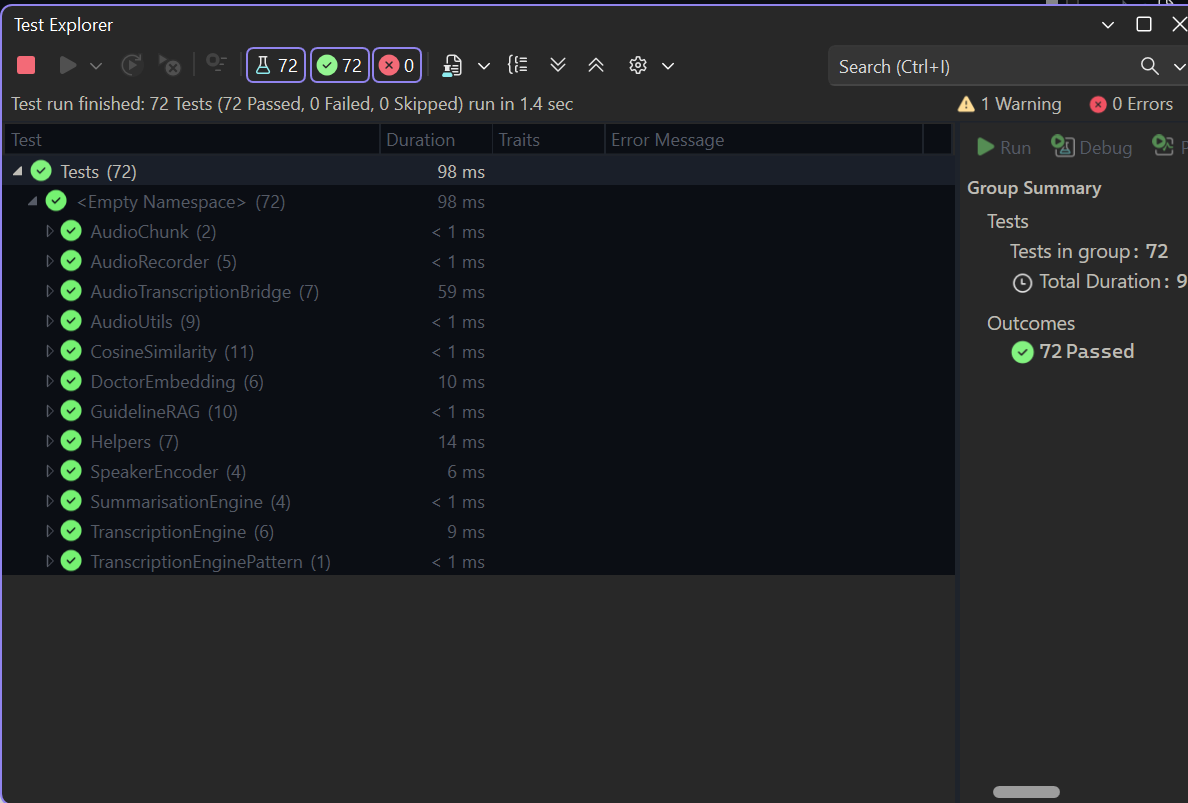
\includegraphics[width=0.5\linewidth]{unittest.png}
    \caption{All 72 unit tests passing within the Visual Studio Text Explorer}
    \label{fig:placeholder}
\end{figure}

\section{Performance Testing}
Performance testing was conducted to verify that the application meets teh latency and responsiveness constraints defined in requirements NF1-4. All tests were executed on the target Intel AI PC.

\begin{table}[H]
\centering
\begin{tabular}{|l|p{6cm}|l|l|}
\hline
\textbf{Req ID} & \textbf{Performance Metric} & \textbf{Target Constraint} & \textbf{Observed Result} \\ \hline
NF1 & Application startup and complete ML model loading into memory & $< 60$ seconds & Med42: $20$s, other models: $4$s \\ \hline
NF2 & Summary generation completion after a 15-minute consultation & $< 90$ seconds & $73$ seconds \\ \hline
NF3 & Semantic search and guidance retrieval over uploaded documents & $< 3$ seconds & $< 1$ second \\ \hline
NF4 & UI Responsiveness during heavy background processing & No freezing/hangs & Completely fluid \\ \hline
\end{tabular}
\caption{Summary of performance testing results against non-functional requirements.}
\label{tab:performance_results}
\end{table}


\subsubsection{Summarisation Inference}
To test the NF2 requirement, a 15 minute mock conversation was conducted with a friend. By recording the time taken for the conversation and inference, we found the result of around 73 seconds for a 15 minute conversation. This can be confirmed by our model benchmarks. During model selection, the longest conversation sample (228 words) required 392 tokens and was inferenced in 6.65 seconds by the Med42-8b int4 model resulting in 58.9 tokens/second or roughly 34 words/second. Extrapolating this to a 15 minute, 2000 word consultation, results in a predicted 58 second inference time.

\subsubsection{Retrieval Latency (NF3)}
This requirement was tested by uploading 3 medical PDFs and pressing "view guidance". On an average of 10 runs, the time taken between pressing "view guidance" and the UI displaying the highlighted guidance within the PDF averaged 2 seconds.

\subsubsection{UI Responsiveness (NF4)}
Throughout all UI testing, the user interface remained responsive with no noticeable delay

\subsection{Accuracy Testing}
\subsubsection{Summarisation}
After selecting Med42 as our summarisation model, the LLM testing framework (TODO link) was re-ran with the \texttt{rescale\_with\_baseline\=False} to provide an individual benchmark over a comparative benchmark. The results provided in \ref{fig:med42_benchmark} demonstrating it is fit for purpose with a precision score of 88\%.

\begin{figure}[H]
    \centering
    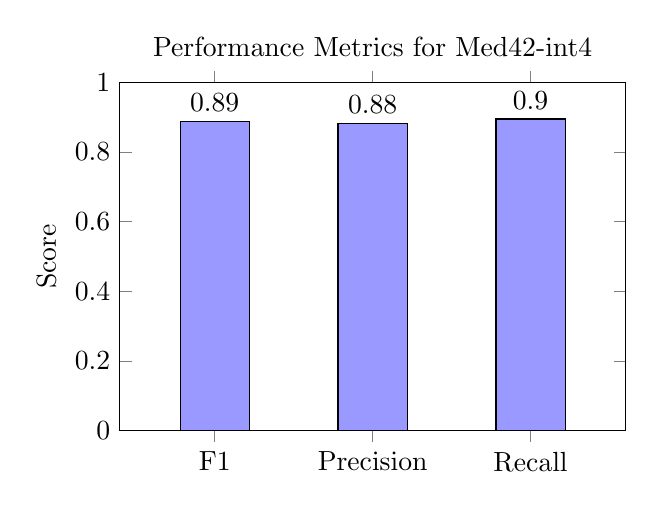
\begin{tikzpicture}
        \begin{axis}[
            ybar,
            title={Performance Metrics for Med42-int4},
            ylabel={Score},
            symbolic x coords={F1, Precision, Recall},
            xtick=data,
            ymin=0.0, ymax=1.0, % Zoomed in slightly to show the differences better
            nodes near coords, % Displays the numbers on top of the bars
            nodes near coords align={vertical},
            bar width=25pt,
            enlarge x limits=0.3, % Adds space on the left and right sides
            width=8cm,
            height=6cm
        ]
        
        \addplot[fill=blue!40] coordinates {
            (F1, 0.888) 
            (Precision, 0.882) 
            (Recall, 0.895)
        };
        
        \end{axis}
    \end{tikzpicture}
    \label{fig:med42_benchmark}
    \caption{Evaluation metrics for the Med42-int4 model.}
\end{figure}

\subsubsection{Transcription}
The accuracy of the transcription in this clinical setting was tested on medical terminology. A glossary of medical terminology published by the European Medicines Agency \cite{ema_medical_terms_simplifier} was used as the ground truth set. This was conducted by running the application and speaking 4 randomly selected words for each starting letter of the alphabet. Once completed, the transcription was viewed and compared against the glossary. To analyse these results, each word was placed into a category of correct, minor inaccuracy (punctuation or American English) and major inaccuracy.

\begin{table}[htbp]
\centering
\begin{tabular}{|c|c|c|c|}
\hline
\textbf{Count} & \textbf{Correct} & \textbf{Inaccuracy} & \textbf{Incorrect} \\
\hline
104 & 93 & 8 & 3 \\
\hline
\end{tabular}
\caption{Transcription results with Whisper-Medium on 104 medical terminology samples}
\label{tab:results}
\end{table}

Generally, the transcription model has a large enough vocabulary to accurately transcribe medical terminology. Common inaccuracies involve incorrect hyphens, American English spelling, and incorrect capitalisation. The incorrectly transcribed words included syncope, fissure and tophi miss-transcribed to sync up, Fisher and trophy. This is likely due to the transcribed words having higher weights within the model due to their popularity compared to the niche medical terminology. Overall an 93\% accuracy on medical terminology is acceptable, especially since the summarisation can infer context. The full results can be examined in Appendix \ref{app:testing_transcription_results}.

\subsubsection{Diarisation}
The speaker diarisation model provides a score from 0-1 on how likely the person speaking is the doctor for a given audio chunk. Empirical testing was conducted to determine what the threshold value should be to decide if the doctor was speaking or someone else. By encoding the doctor as person myself, 1 minute of audio was captured each for myself and a friend reading the introduction to this dissertation. The results showed the average doctor score to be 0.76, with the patient score as 0.54, leading to the threshold value set at 0.7.

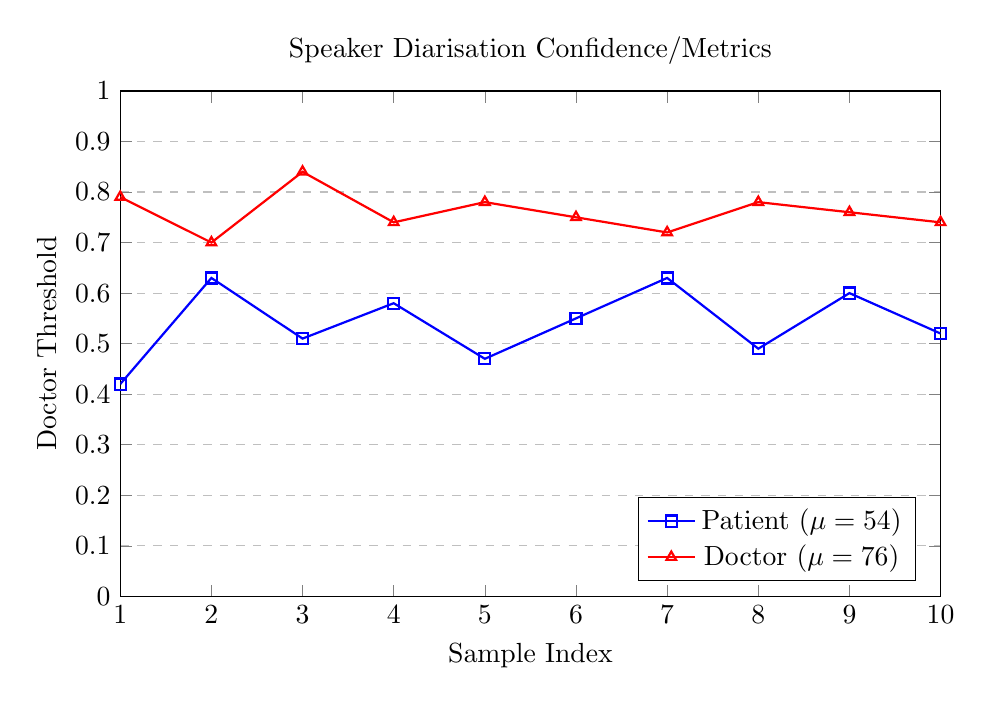
\begin{tikzpicture}
\begin{axis}[
    title={Speaker Diarisation Confidence/Metrics},
    xlabel={Sample Index},
    ylabel={Doctor Threshold},
    xmin=1, xmax=10,
    ymin=0, ymax=1, 
    xtick={1,2,3,4,5,6,7,8,9,10},
    ytick={0, 0.1, 0.2, 0.3, 0.4, 0.5, 0.6, 0.7, 0.8, 0.9, 1.0},
    legend pos=south east,
    ymajorgrids=true,
    grid style=dashed,
    width=12cm,
    height=8cm
]

\addplot[
    color=blue,
    mark=square,
    thick
]
coordinates {
    (1, 0.42)
    (2, 0.63)
    (3, 0.51)
    (4, 0.58)
    (5, 0.47)
    (6, 0.55)
    (7, 0.63)
    (8, 0.49)
    (9, 0.60)
    (10, 0.52)
};
\addlegendentry{Patient ($\mu = 54$)}

\addplot[
    color=red,
    mark=triangle,
    thick
]
coordinates {
    (1, 0.79)
    (2, 0.70)
    (3, 0.84)
    (4, 0.74)
    (5, 0.78)
    (6, 0.75)
    (7, 0.72)
    (8, 0.78)
    (9, 0.76)
    (10, 0.74)
};
\addlegendentry{Doctor ($\mu = 76$)}

\end{axis}
\end{tikzpicture}

The full results can be examined here \ref{app:speaker_diarisation_results}

\subsubsection{Guidelines Retrieval}
Due to the custom retrieval pipeline implementation, testing with a ground truth PDF dataset is unfeasible. Without a found ground truth set, no quantitative testing or results can be generated. That being said, qualitative testing was completed. Generally speaking, the retrieved guidance was accurate, however was highly dependent on the specificity of the guidance PDFs uploaded. General documents laying out a disease progression or advice for trivial diseases provided little valuable insights. Very specific guidance documents were highly effective at retrieving medical guidance that is important to the conversation.

\section{UI Testing}
User interface testing began by testing every state transition in the application to ensure that the state management system was functional. Next, persistent data such as the doctor's voice embedding, appraisals and uploaded guidance was loaded, then checked for their presence after an application restart. All tests passed, while the UI stayed responsive and in the state we were expecting. A full list of test cases is in the appendix \ref{app:UI_test}

\section{User Acceptance Testing}
Throughout the project, 5 demonstrations and 2 trials of the application were conducted with Dr Atia Rafiq and Dr Tazeen Ahmed. At a UCL hosted AI conference, I trialled the application by mocking a consultation with Dr Tazeen Ahmed where she used the application as if she was conducting a real consultation. The application took no explanation on how to use and the consultation was successfully carried out resulting in a successful user acceptance test(TODO requirement). She expressed her enthusiasm with the project and commented that this application would "save her lots of time taking notes and reviewing consultations throughout the day". She further commented that the appraisals system would be "highly beneficial" for training GPs. She also provided feedback regarding the prompt, requesting the prompt to use the "the patient says" and "the doctor suggested" formats which were integrated after the event.

On a video call with Dr Atia Rafiq, I demonstrated the application. She noted that the user interface looked easy to use and had an appeasing design and that the application would be very useful to her and her trainee GPs. She added a further recommendation to create the appraisals component to allow note taking and commentary on conversations to demonstrate learning that was conducted post-consultation.




